\section{Results}
\subsection{Initial Code, Importance Sampling, and Statistical Analysis}
Figure \ref{fig:naive-nin} show a clear trend that

\begin{figure}[h]
\hspace{-2.8cm}
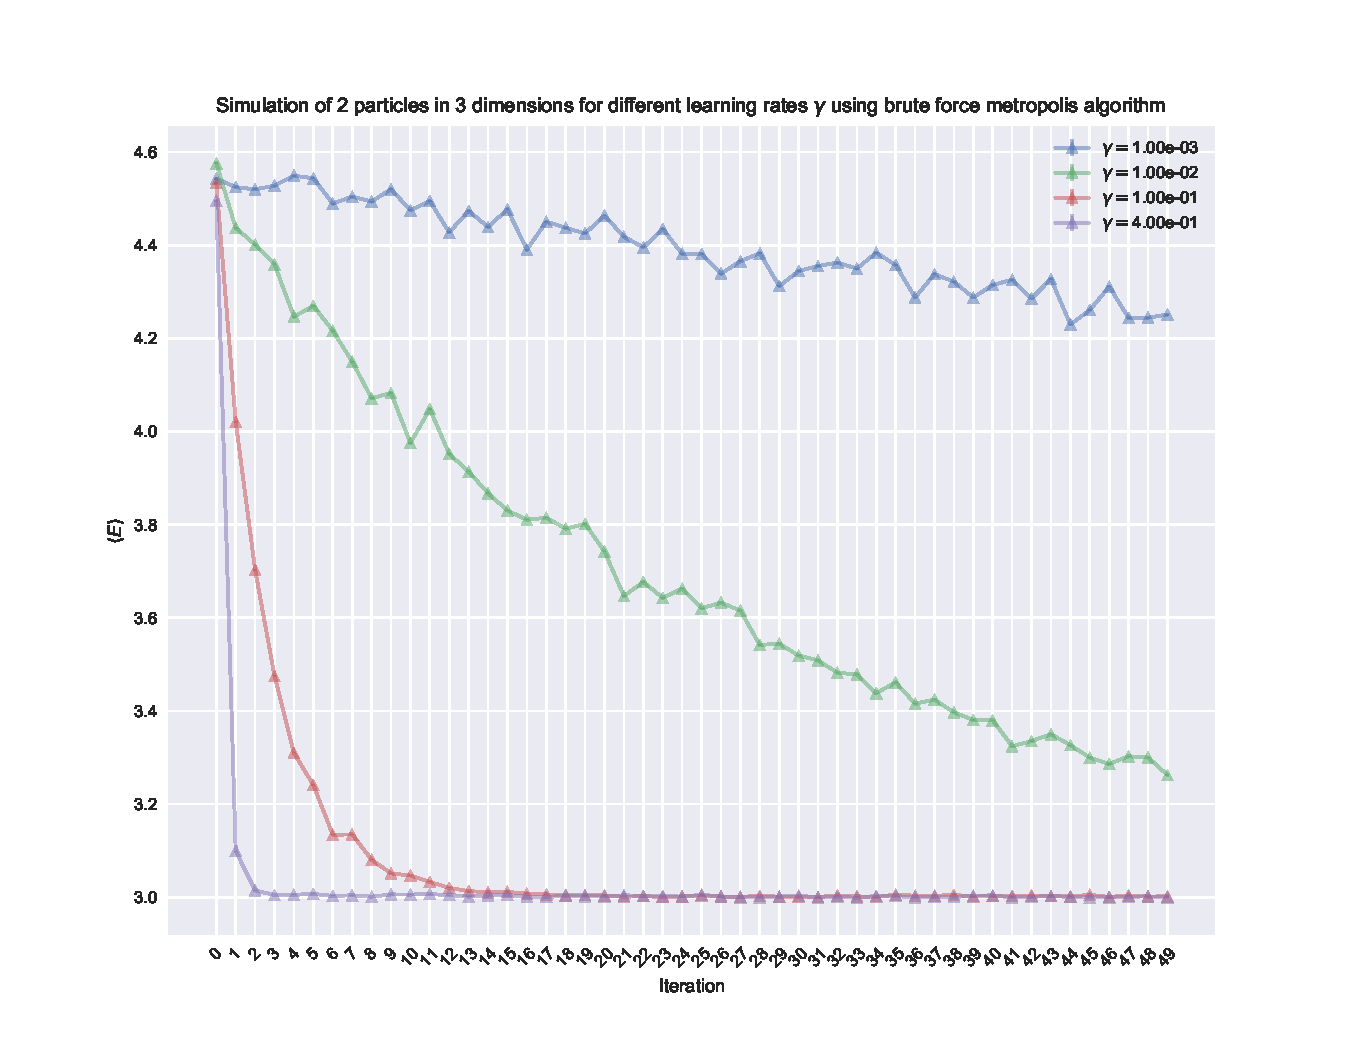
\includegraphics[width = \paperwidth]{figures/naive_2p_3d.pdf}
\caption{Plot of simulation with 2 particles in 3 dimensions with varied learning rates $\gamma$, using brute force metropolis sampling.
			2 hidden nodes were used.
			For detailed values on energy, variance, and CPU-time per mc-cycle, see table \ref{tab:naive-nin}}
\label{fig:naive-nin}
\end{figure}

\begin{table}[h]
\begin{tabular}{l c c}
	Mean time per mc-cycle & &$5.88\cdot10^{-5}$ s \\
	\hline
	$\gamma$ & $\expect{E_L}$ a.u & Mean Variance $\sqrt{\sigma}$\\
	\hline
	$1\cdot10^{-3}$ & $4.25$ & $2.99\cdot10^{-2}$ \\
	$1\cdot10^{-2}$ & $3.26$ & $1.48\cdot10^{-2}$ \\
	$1\cdot10^{-1}$ & $3.002$ & $1.67\cdot10^{-3}$ \\
	$4\cdot10^{-1}$ & $3.000$ & $1.23\cdot10^{-3}$ \\
\end{tabular}
\label{tab:naive-nin}
\caption{Table of learning rates $\gamma$ and corresponding expectation values obtained for the local energy $E_L$ with variance, for brute force metropolis sampling.
		Mean CPU-time per monte-carlo cycle across all iterations at the top. 4 hidden nodes were used.
	For corresponding plot, see figure \ref{fig:naive-nin}}
\end{table}

\begin{figure}[h]
\hspace{-2.8cm}
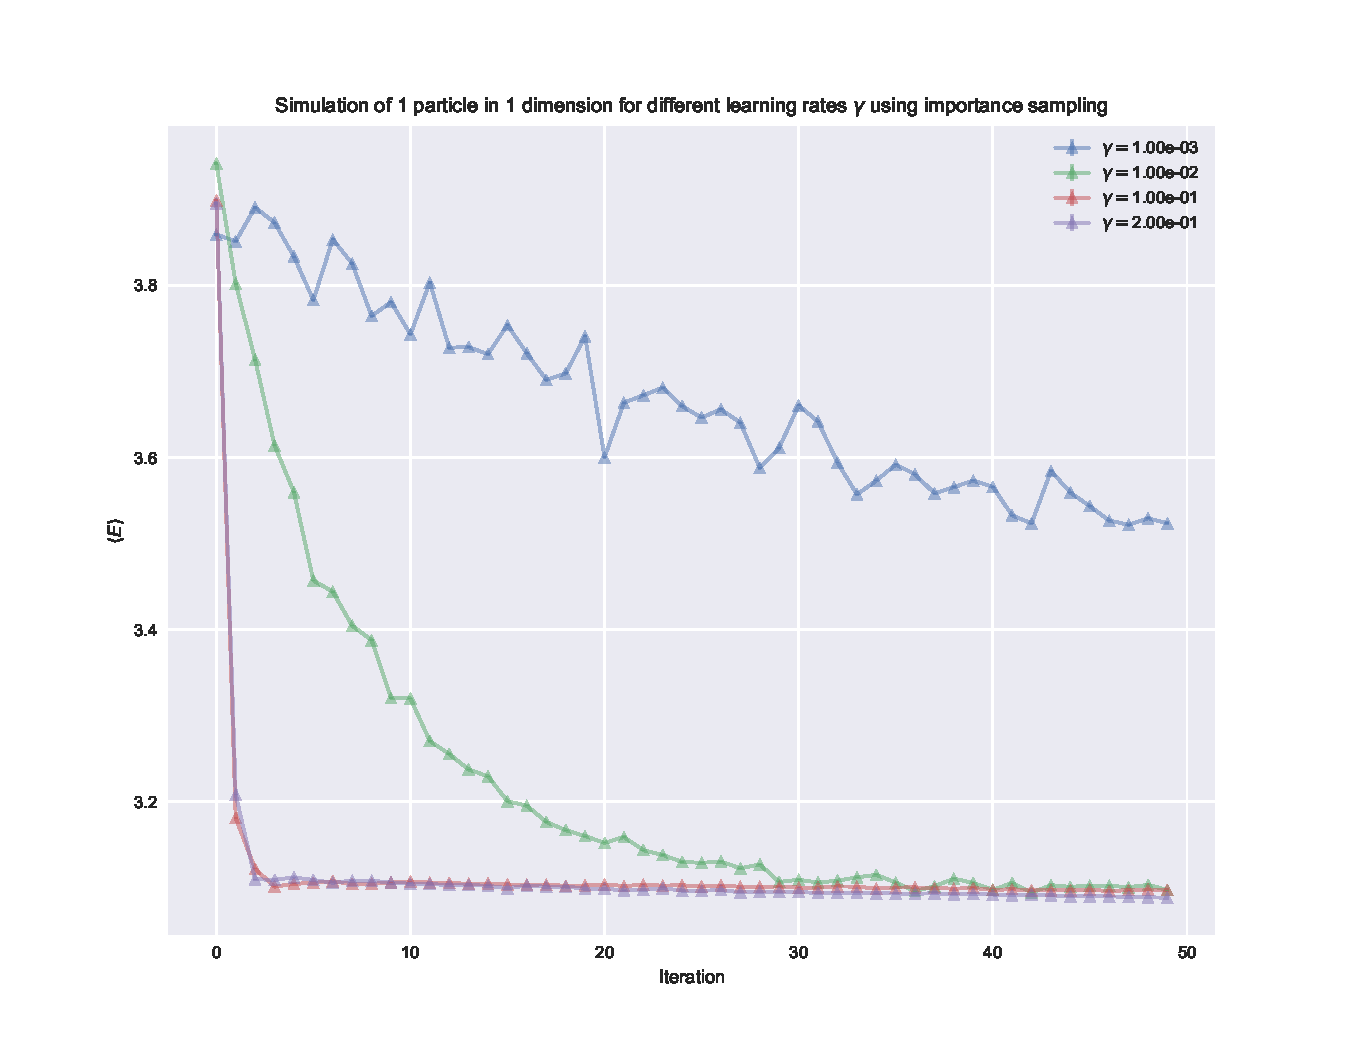
\includegraphics[width = \paperwidth]{figures/importance_2p_3d.pdf}
\caption{Plot of simulation with 2 particles in 3 dimensions with varied learning rates $\gamma$, using brute force metropolis sampling.
			For detailed values on energy, variance, and CPU-time per mc-cycle, see table \ref{tab:importance-nin-gamma}}
\label{fig:importance-nin-gamma}
\end{figure}

\begin{table}[h]
\begin{tabular}{l c c}
	Mean time per mc-cycle & &$4.81\cdot10^{-4}$ s \\
	\hline
	$\gamma$ & $\expect{E_L}$ a.u & Mean Variance $\sqrt{\sigma}$\\
	\hline
	$1\cdot10^{-3}$ & $3.45$ & $2.22\cdot10^{-2}$ \\
	$1\cdot10^{-2}$ & $3.262$ & $4.08\cdot10^{-3}$ \\
	$1\cdot10^{-1}$ & $3.264$ & $1.52\cdot10^{-3}$ \\
	$2\cdot10^{-1}$ & $3.1364$ & $9.41\cdot10^{-4}$ \\
\end{tabular}
\label{tab:importance-nin-gamma}
\caption{Table of learning rates $\gamma$ and corresponding expectation values obtained for the local energy $E_L$ with variance, for importance sampling.
		Mean CPU-time per monte-carlo cycle across all iterations at the top. 4 hidden nodes were used.
	For corresponding plot, see figure \ref{fig:importance-nin-gamma}}
\end{table}

\begin{figure}[h]
\hspace{-2.8cm}
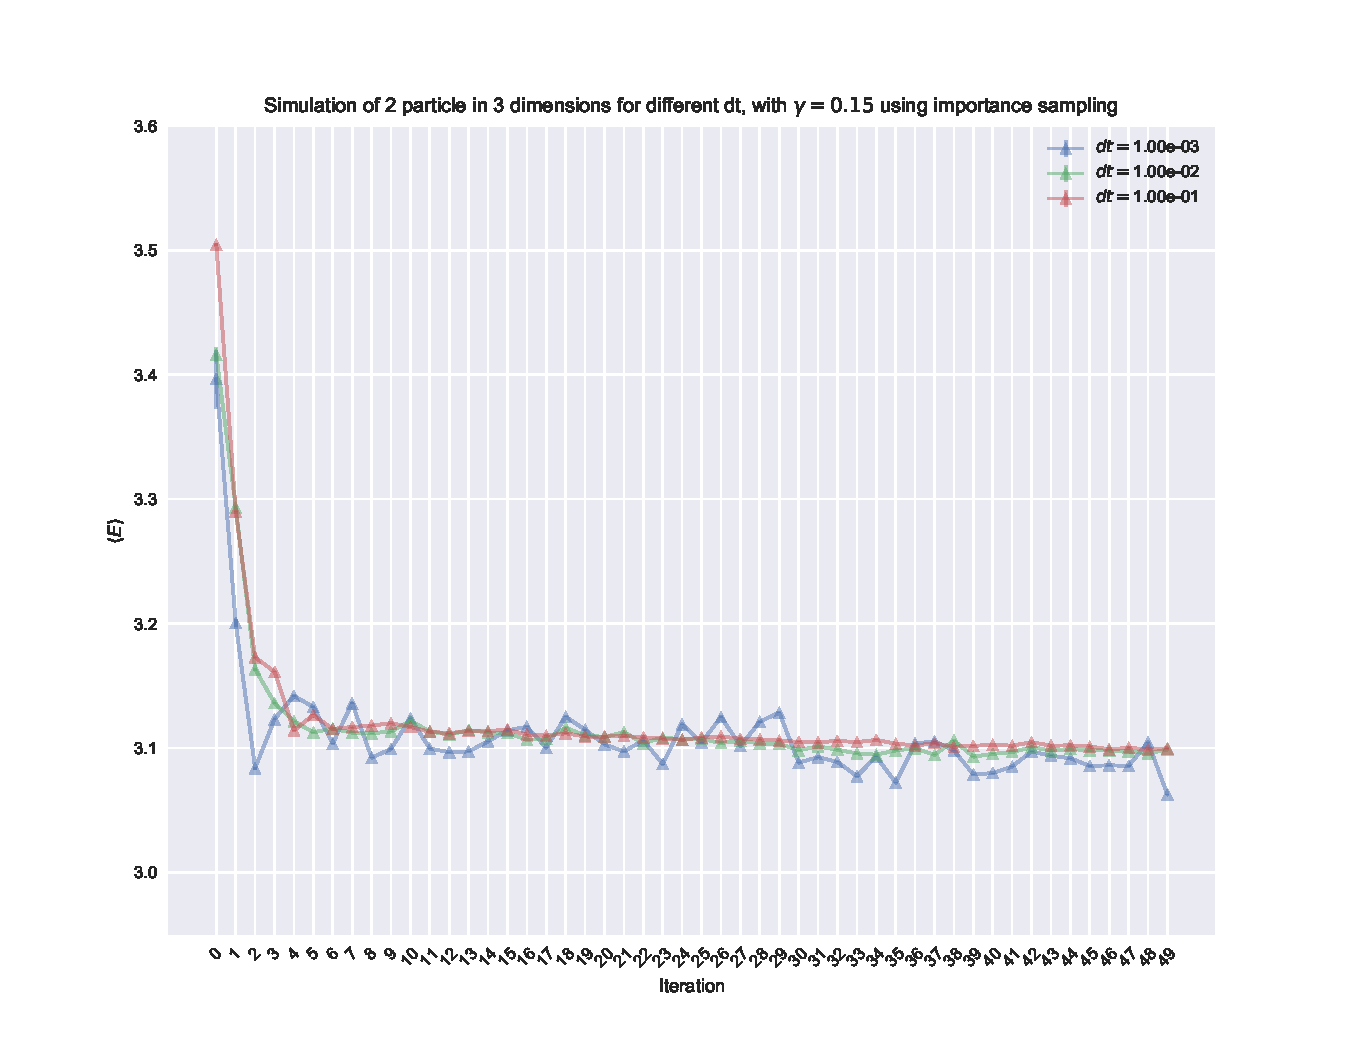
\includegraphics[width = \paperwidth]{figures/importance_2p_3d_dt.pdf}
\caption{Plot of simulation with 2 particles in 3 dimensions with varied learning rates $\gamma$, using brute force metropolis sampling.
			For detailed values on energy, variance, and CPU-time per mc-cycle, see table \ref{tab:importance-nin-dt}}
\label{fig:importance-nin-dt}
\end{figure}

\begin{table}[h]
\begin{tabular}{l c c}
	Mean time per mc-cycle & & $5.24\cdot10^{-4}$ s \\
	\hline
	$dt$ & $\expect{E_L}$ a.u & Mean Variance $\sqrt{\sigma}$\\
	\hline
	$1\cdot10^{-3}$ & $3.062$ & $9.18\cdot10^{-3}$ \\
	$1\cdot10^{-2}$ & $3.098$ & $3.43\cdot10^{-3}$ \\
	$1\cdot10^{-1}$ & $3.099$ & $1.13\cdot10^{-3}$ \\
\end{tabular}
\label{tab:importance-nin-dt}
\caption{Table of timesteps $dt$ and corresponding expectation values obtained for the local energy $E_L$ with variance, for importance sampling.
		Mean CPU-time per monte-carlo cycle across all iterations at the top.
	For corresponding plot, see figure \ref{fig:importance-nin-dt}}
\end{table}

